% Options for packages loaded elsewhere
\PassOptionsToPackage{unicode}{hyperref}
\PassOptionsToPackage{hyphens}{url}
%
\documentclass[
]{article}
\usepackage{amsmath,amssymb}
\usepackage{iftex}
\ifPDFTeX
  \usepackage[T1]{fontenc}
  \usepackage[utf8]{inputenc}
  \usepackage{textcomp} % provide euro and other symbols
\else % if luatex or xetex
  \usepackage{unicode-math} % this also loads fontspec
  \defaultfontfeatures{Scale=MatchLowercase}
  \defaultfontfeatures[\rmfamily]{Ligatures=TeX,Scale=1}
\fi
\usepackage{lmodern}
\ifPDFTeX\else
  % xetex/luatex font selection
\fi
% Use upquote if available, for straight quotes in verbatim environments
\IfFileExists{upquote.sty}{\usepackage{upquote}}{}
\IfFileExists{microtype.sty}{% use microtype if available
  \usepackage[]{microtype}
  \UseMicrotypeSet[protrusion]{basicmath} % disable protrusion for tt fonts
}{}
\makeatletter
\@ifundefined{KOMAClassName}{% if non-KOMA class
  \IfFileExists{parskip.sty}{%
    \usepackage{parskip}
  }{% else
    \setlength{\parindent}{0pt}
    \setlength{\parskip}{6pt plus 2pt minus 1pt}}
}{% if KOMA class
  \KOMAoptions{parskip=half}}
\makeatother
\usepackage{xcolor}
\usepackage[margin=1in]{geometry}
\usepackage{color}
\usepackage{fancyvrb}
\newcommand{\VerbBar}{|}
\newcommand{\VERB}{\Verb[commandchars=\\\{\}]}
\DefineVerbatimEnvironment{Highlighting}{Verbatim}{commandchars=\\\{\}}
% Add ',fontsize=\small' for more characters per line
\usepackage{framed}
\definecolor{shadecolor}{RGB}{248,248,248}
\newenvironment{Shaded}{\begin{snugshade}}{\end{snugshade}}
\newcommand{\AlertTok}[1]{\textcolor[rgb]{0.94,0.16,0.16}{#1}}
\newcommand{\AnnotationTok}[1]{\textcolor[rgb]{0.56,0.35,0.01}{\textbf{\textit{#1}}}}
\newcommand{\AttributeTok}[1]{\textcolor[rgb]{0.13,0.29,0.53}{#1}}
\newcommand{\BaseNTok}[1]{\textcolor[rgb]{0.00,0.00,0.81}{#1}}
\newcommand{\BuiltInTok}[1]{#1}
\newcommand{\CharTok}[1]{\textcolor[rgb]{0.31,0.60,0.02}{#1}}
\newcommand{\CommentTok}[1]{\textcolor[rgb]{0.56,0.35,0.01}{\textit{#1}}}
\newcommand{\CommentVarTok}[1]{\textcolor[rgb]{0.56,0.35,0.01}{\textbf{\textit{#1}}}}
\newcommand{\ConstantTok}[1]{\textcolor[rgb]{0.56,0.35,0.01}{#1}}
\newcommand{\ControlFlowTok}[1]{\textcolor[rgb]{0.13,0.29,0.53}{\textbf{#1}}}
\newcommand{\DataTypeTok}[1]{\textcolor[rgb]{0.13,0.29,0.53}{#1}}
\newcommand{\DecValTok}[1]{\textcolor[rgb]{0.00,0.00,0.81}{#1}}
\newcommand{\DocumentationTok}[1]{\textcolor[rgb]{0.56,0.35,0.01}{\textbf{\textit{#1}}}}
\newcommand{\ErrorTok}[1]{\textcolor[rgb]{0.64,0.00,0.00}{\textbf{#1}}}
\newcommand{\ExtensionTok}[1]{#1}
\newcommand{\FloatTok}[1]{\textcolor[rgb]{0.00,0.00,0.81}{#1}}
\newcommand{\FunctionTok}[1]{\textcolor[rgb]{0.13,0.29,0.53}{\textbf{#1}}}
\newcommand{\ImportTok}[1]{#1}
\newcommand{\InformationTok}[1]{\textcolor[rgb]{0.56,0.35,0.01}{\textbf{\textit{#1}}}}
\newcommand{\KeywordTok}[1]{\textcolor[rgb]{0.13,0.29,0.53}{\textbf{#1}}}
\newcommand{\NormalTok}[1]{#1}
\newcommand{\OperatorTok}[1]{\textcolor[rgb]{0.81,0.36,0.00}{\textbf{#1}}}
\newcommand{\OtherTok}[1]{\textcolor[rgb]{0.56,0.35,0.01}{#1}}
\newcommand{\PreprocessorTok}[1]{\textcolor[rgb]{0.56,0.35,0.01}{\textit{#1}}}
\newcommand{\RegionMarkerTok}[1]{#1}
\newcommand{\SpecialCharTok}[1]{\textcolor[rgb]{0.81,0.36,0.00}{\textbf{#1}}}
\newcommand{\SpecialStringTok}[1]{\textcolor[rgb]{0.31,0.60,0.02}{#1}}
\newcommand{\StringTok}[1]{\textcolor[rgb]{0.31,0.60,0.02}{#1}}
\newcommand{\VariableTok}[1]{\textcolor[rgb]{0.00,0.00,0.00}{#1}}
\newcommand{\VerbatimStringTok}[1]{\textcolor[rgb]{0.31,0.60,0.02}{#1}}
\newcommand{\WarningTok}[1]{\textcolor[rgb]{0.56,0.35,0.01}{\textbf{\textit{#1}}}}
\usepackage{longtable,booktabs,array}
\usepackage{calc} % for calculating minipage widths
% Correct order of tables after \paragraph or \subparagraph
\usepackage{etoolbox}
\makeatletter
\patchcmd\longtable{\par}{\if@noskipsec\mbox{}\fi\par}{}{}
\makeatother
% Allow footnotes in longtable head/foot
\IfFileExists{footnotehyper.sty}{\usepackage{footnotehyper}}{\usepackage{footnote}}
\makesavenoteenv{longtable}
\usepackage{graphicx}
\makeatletter
\def\maxwidth{\ifdim\Gin@nat@width>\linewidth\linewidth\else\Gin@nat@width\fi}
\def\maxheight{\ifdim\Gin@nat@height>\textheight\textheight\else\Gin@nat@height\fi}
\makeatother
% Scale images if necessary, so that they will not overflow the page
% margins by default, and it is still possible to overwrite the defaults
% using explicit options in \includegraphics[width, height, ...]{}
\setkeys{Gin}{width=\maxwidth,height=\maxheight,keepaspectratio}
% Set default figure placement to htbp
\makeatletter
\def\fps@figure{htbp}
\makeatother
\setlength{\emergencystretch}{3em} % prevent overfull lines
\providecommand{\tightlist}{%
  \setlength{\itemsep}{0pt}\setlength{\parskip}{0pt}}
\setcounter{secnumdepth}{5}
\usepackage{booktabs}
\usepackage{booktabs}
\usepackage{longtable}
\usepackage{array}
\usepackage{multirow}
\usepackage{wrapfig}
\usepackage{float}
\usepackage{colortbl}
\usepackage{pdflscape}
\usepackage{tabu}
\usepackage{threeparttable}
\usepackage{threeparttablex}
\usepackage[normalem]{ulem}
\usepackage{makecell}
\usepackage{xcolor}
\ifLuaTeX
  \usepackage{selnolig}  % disable illegal ligatures
\fi
\usepackage[]{natbib}
\bibliographystyle{plainnat}
\usepackage{bookmark}
\IfFileExists{xurl.sty}{\usepackage{xurl}}{} % add URL line breaks if available
\urlstyle{same}
\hypersetup{
  pdftitle={Tree phenology analysis with R},
  pdfauthor={Jacqueline Wingen},
  hidelinks,
  pdfcreator={LaTeX via pandoc}}

\title{Tree phenology analysis with R}
\author{Jacqueline Wingen}
\date{27 Oktober 2024}

\begin{document}
\maketitle

{
\setcounter{tocdepth}{2}
\tableofcontents
}
\section{Introduction}\label{introduction}

Hi, my name is Jacqueline. I'm a master's student in crop sciences at the \href{}{University of Bonn}. This is my learning logbook for the module ``Tree phenology analysis with R''. This module provides an overview of methods to study the impact of climate and climate change on tree phenology. It is designed for those who may not yet be familiar with phenology or how to analyze climate change effects, but it also aims to offer new insights for those with existing knowledge in these areas. Initially developed for M.Sc. students in Crop Science and Agricultural Science and Resource Management in the Tropics and Subtropics (ARTS) at the \href{https://www.uni-bonn.de/en}{University of Bonn}, the material is accessible to anyone interested.


\includegraphics{images/chillR_hexSticker.png}

The content begins with an introduction to phenology (with a special emphasis on dormancy) as well as an overview of climate change. It then focuses heavily on the practical application of the \texttt{chillR} package for R. This tool has been continuously developed since 2013 by \href{https://www.gartenbauwissenschaft.uni-bonn.de/author/prof.-dr.-eike-luedeling/}{Eike Lüdeling}, head of the \href{https://inresgb-lehre.iaas.uni-bonn.de/}{HortiBonn research group} at the \href{https://www.inres.uni-bonn.de/de}{Institute of Crop Science and Resource Conservation (INRES)} at the \href{https://www.uni-bonn.de/en}{University of Bonn}, to support this type of analysis.

\subsection{Learning goals}\label{learning-goals}

This course will offer the following skills and experiences:

\begin{itemize}
\tightlist
\item
  Knowledge about phenology
\item
  Knowledge about tree dormancy
\item
  Understanding of climate change impact projection methods
\item
  Appreciation for the importance of risks and uncertainty in climate change projection
\item
  Understanding of how to use some staple tools of R code development
\item
  Ability to use \texttt{chillR} functions for climate change impact projection
\item
  Ability to use \texttt{chillR} functions for tree phenology analysis
\item
  Understanding and ability to use the PhenoFlex dormancy analysis framework
\end{itemize}

\section{The tools}\label{the-tools}

This course is designed to provide knowledge about tree phenology, climate change, and related topics, along with hands-on exercises to demonstrate the functionalities of the \texttt{chillR} package. It is recommended to document everything learned in a \texttt{learning\ logbook}. To engage in these practical components effectively, various tools are required. Since \texttt{chillR} is an R package, using \href{https://www.r-project.org/}{R}, preferably through the \href{https://posit.co/download/rstudio-desktop/}{RStudio} interface, will be necessary.

Although it is possible to run RStudio on a local computer and save files directly on the hard drive, this approach differs from the methods commonly used by professional programmers. To align with standard programming practices, familiarity with certain code development tools is essential. This course will therefore cover the basics of using \href{https://git-scm.com/}{Git} and \href{https://github.com/}{GitHub}, which are valuable tools for organizing, securing, and sharing code. Additionally, proper documentation techniques in R will be introduced, focusing on creating well-structured, professional reports using \href{https://rmarkdown.rstudio.com/}{RMarkdown}. While these tools may seem complex at first, their usefulness is likely to become clearer as they are used throughout the module.

\href{https://inresgb-lehre.iaas.uni-bonn.de/author/dr.-cory-whitney/}{Dr.~Cory Whitney}, a researcher at HortiBonn, has volunteered to create tutorial videos to provide an introduction to these tools.

\subsection{R and RStudio}\label{r-and-rstudio}

The first video \emph{Using R and RStudio} demonstrates how to install and run \href{https://www.r-project.org/}{R} and \href{https://posit.co/download/rstudio-desktop/}{RStudio}:

\subsection{Git and Github}\label{git-and-github}

The next video Using \emph{Git and Github} explores the programming version control environment \href{https://git-scm.com/}{Git} and the interface \href{https://github.com/}{GitHub}, which is used to access these features:

\subsection{Rmarkdown}\label{rmarkdown}

In the last video \emph{Using R Mardown}, R Markdown will be examined, a powerful tool that enables the creation of sophisticated reports, websites, and more from R code. An example is currently being viewed, as this website was produced using R Markdown

\section{Tree dormancy}\label{tree-dormancy}

This chapter is presented by \href{https://scholar.google.de/citations?hl=de&user=MTmTnnsAAAAJ}{Dr.~Erica Fadón}, a researcher at \href{https://inresgb-lehre.iaas.uni-bonn.de/author/dr.-erica-fadon-adrian/}{HortiBonn from 2018 to 2021}, who explores dormancy in temperate fruit trees. This topic remains complex and has many unanswered questions. A central question for researchers is, ``How do trees know when to flower?'' Although it seems clear that trees bloom in spring, the reality is more complicated. This chapter provides a better understanding of dormancy and demonstrates how to use the \texttt{chillR} tool to predict flowering times, even in the face of challenges posed by global warming.

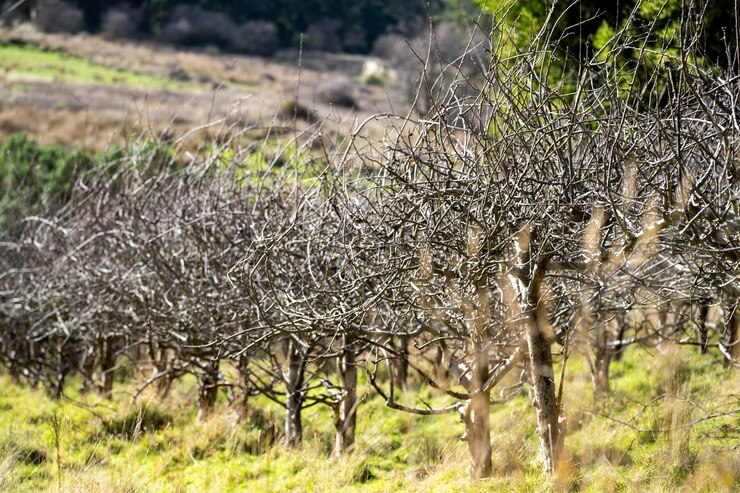
\includegraphics{images/dormant-grown-apple-tree-that-need-pruning-field-australia_866797-3589.jpg}

\subsection{Learning goals}\label{learning-goals-1}

\begin{itemize}
\tightlist
\item
  Learn about dormancy in temperate fruit trees
\item
  Be able to identify the phenological stages of a fruit tree and understand phenology data sets
\item
  Describe and compare the two methodologies (empirical and statistical) to identify the chilling and forcing periods of a certain cultivar
\end{itemize}

\subsection{Introduction to dormancy}\label{introduction-to-dormancy}

Tree dormancy is a state of reduced activity that occurs when environmental conditions are unfavorable, especially during winter. This state acts as a survival strategy, helping trees withstand extreme temperatures, water shortages, and other stress factors. During dormancy, trees slow down or stop their growth to conserve energy and avoid damage. Dormancy is a continuous process divided into three phases:

\begin{itemize}
\tightlist
\item
  \textbf{Dormancy Establishment}
\item
  \textbf{Endo-Dormancy}
\item
  \textbf{Eco-Dormancy}
\end{itemize}

Dormancy establishment is the process where temperate trees transition from active growth in summer to a dormant state in autumn. This shift is mainly triggered by shorter daylight hours and decreasing temperatures, causing buds to form, growth to stop, and leaves to fall. The importance of these factors varies by species, with some trees responding more to day length and others to temperature.

Endo-dormancy is a phase of dormancy controlled by the plant's internal factors, where growth is suppressed even under favorable conditions. It requires a period of cold exposure (chilling) to release the buds from this state, preventing premature growth during temporary warm spells in winter. Low temperatures are the main trigger for breaking endo-dormancy, while the role of light (photoperiod) is still uncertain.

Eco-dormancy is the phase after endo-dormancy, where buds have regained their ability to grow but remain inactive due to unfavorable environmental conditions, mainly low temperatures. During this phase, growth is on hold until warmer temperatures trigger it. Heat accumulation is needed to resume growth. Eco-dormancy ends when enough heat has been accumulated, leading to visible growth changes, typically in late winter or early spring.

The below video \emph{Introduction to dormancy} by \href{https://scholar.google.de/citations?hl=de&user=MTmTnnsAAAAJ}{Dr.~Erica Fadón} gives the basic knowledge of this dormancy phases and processes that regulate dormancy.

\subsection{Dormancy physiology}\label{dormancy-physiology}

Dormancy as a whole is the result of complex interactions between numerous physiological processes that occur in different parts of the tree, such as buds, twigs, meristems, and vascular tissues. We divide these processes into four main themes:

\begin{itemize}
\tightlist
\item
  \textbf{Transport:} occurs at both the whole-plant and cellular levels
\item
  \textbf{Phytohormone Dynamics:} behavior and levels of plant hormones during dormancy
\item
  \textbf{Genetic and Epigenetic Regulation:} how genetic factors and their modifications influence dormancy
\item
  \textbf{Dynamics of Nonstructural Carbohydrates:} changes in carbohydrate levels that affect dormancy
\end{itemize}

The following figure from the study \href{https://www.mdpi.com/2073-4395/10/2/241\#}{\emph{``A conceptual framework for Winter Dormancy in Deciduous Trees''}} by Fadón et al.~(2015) presents a conceptual framework of winter dormancy in deciduous trees and summarizes the three dormancy phases along with their respective physiological processes.

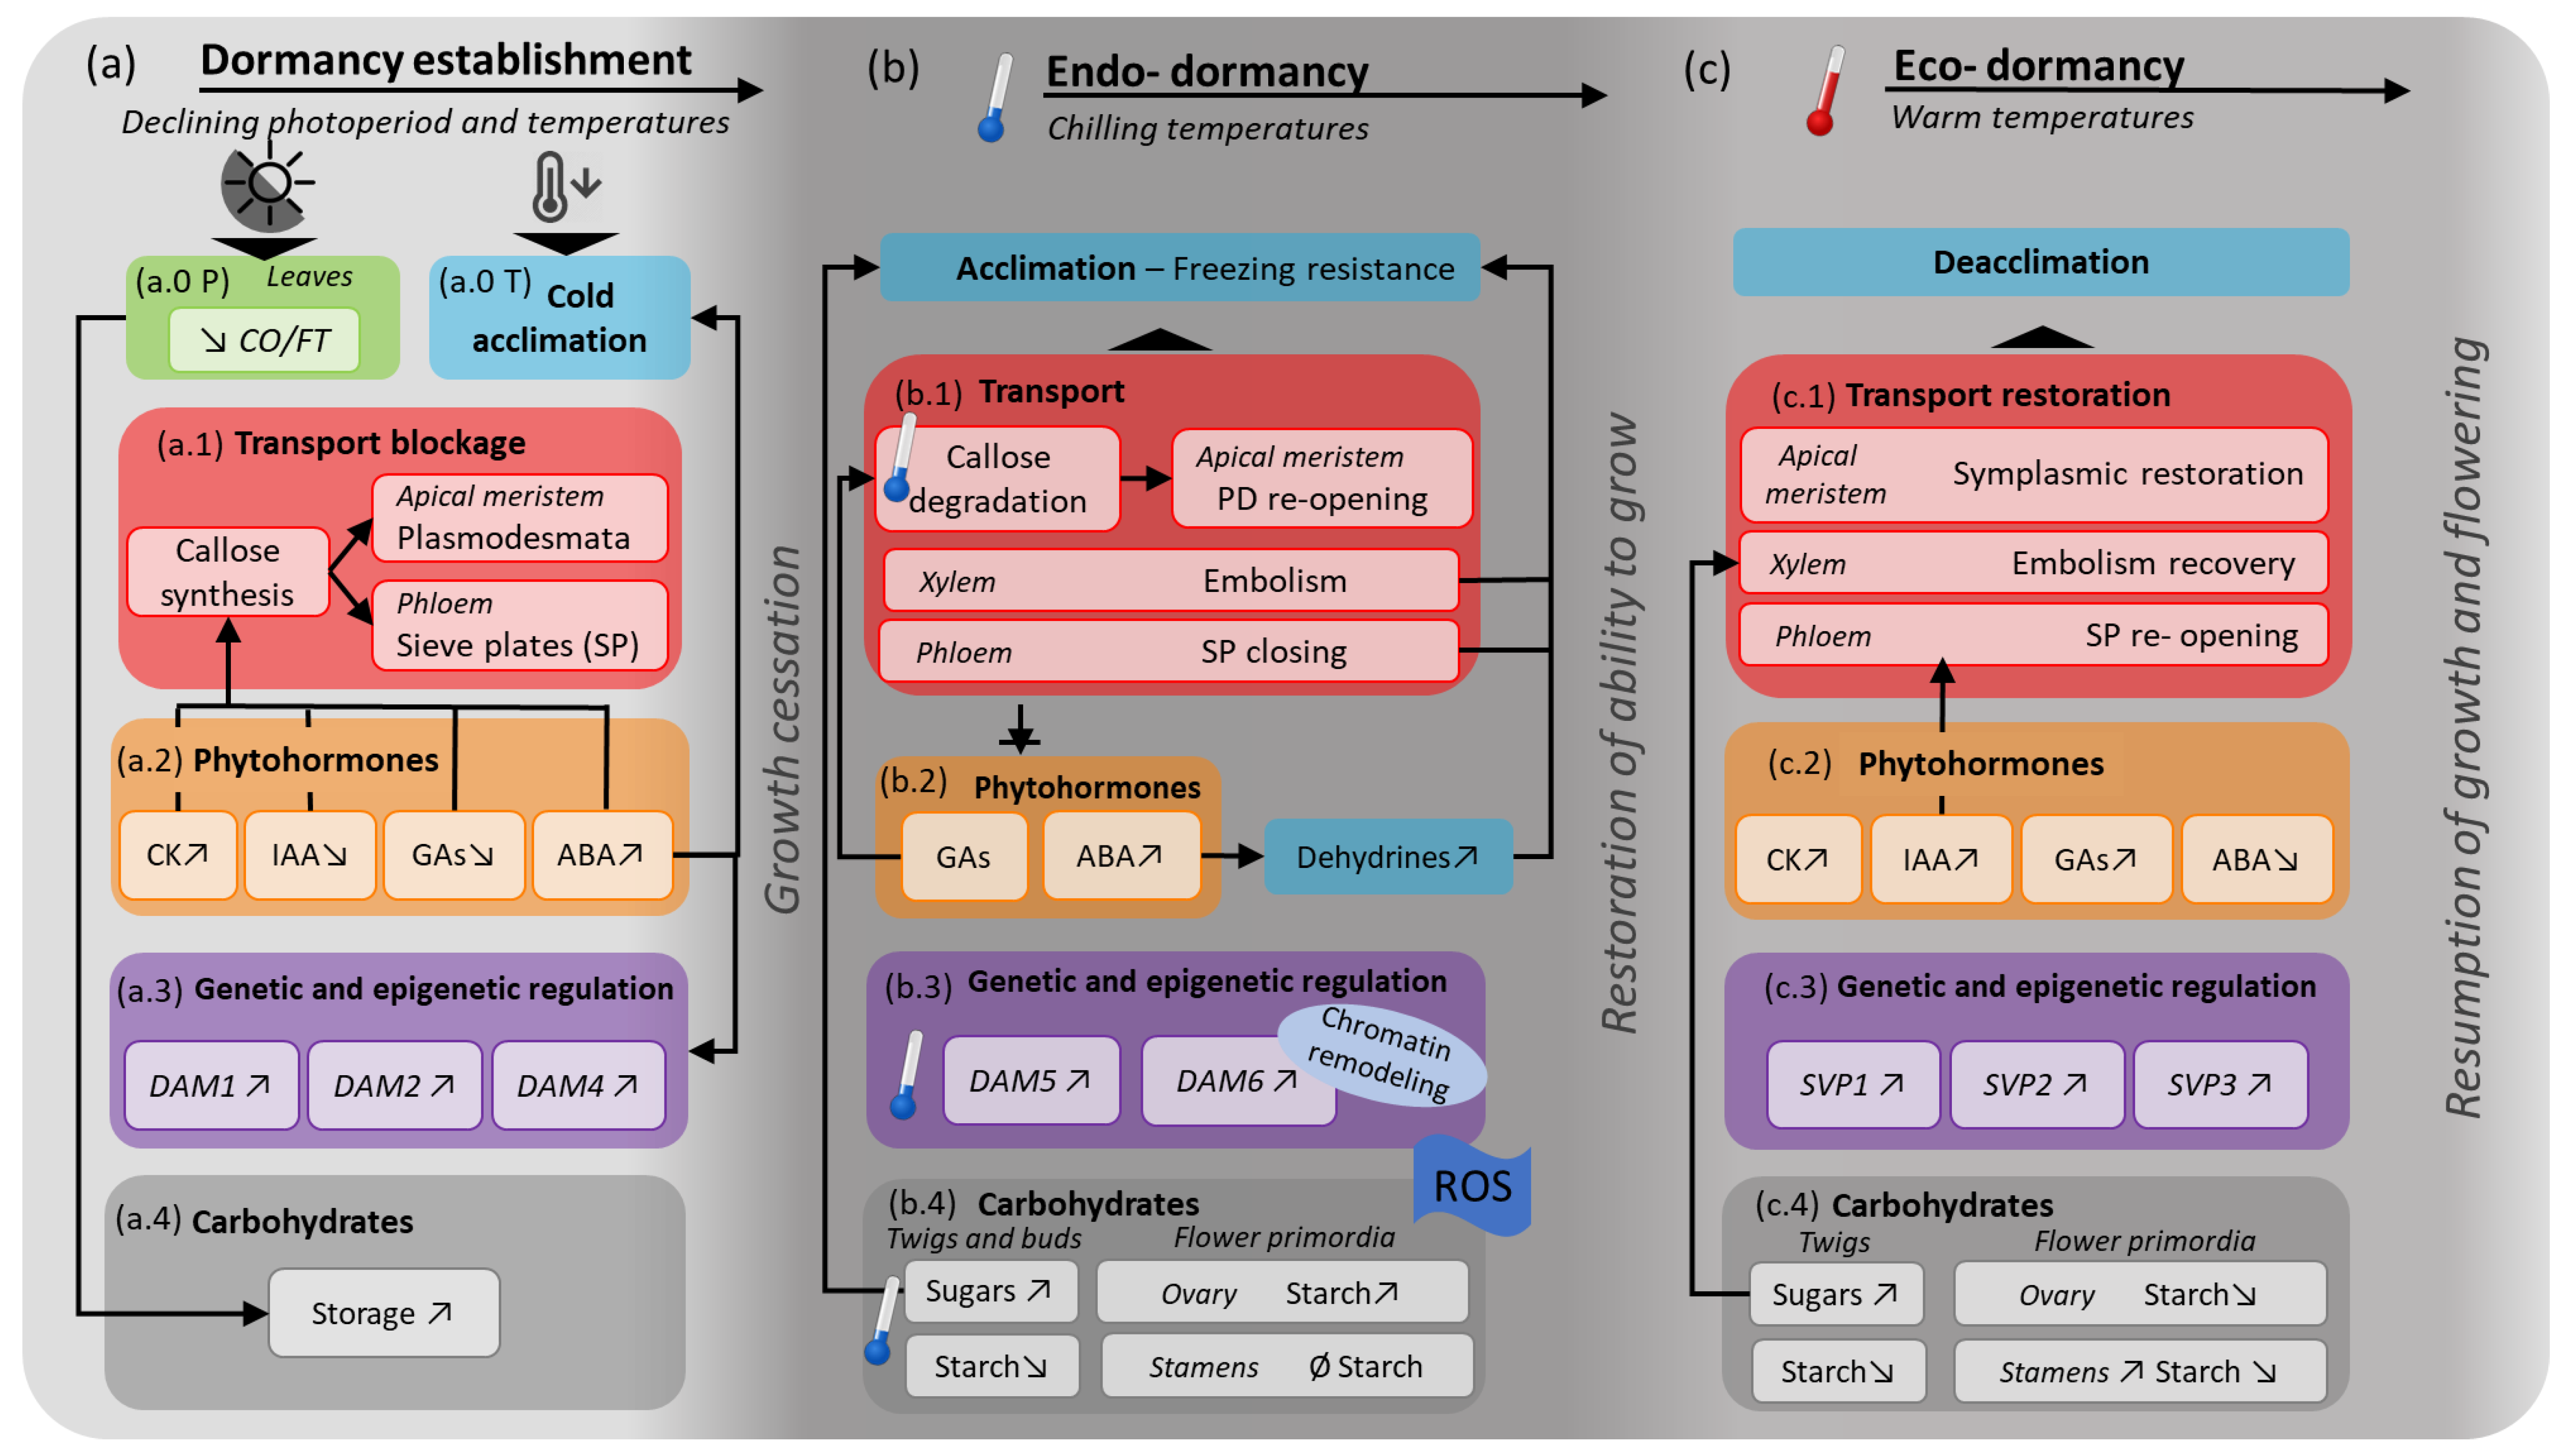
\includegraphics{images/agronomy-10-00241-g003.png}

All the processes depicted are explained in detail in the video below, \emph{Dormancy Physiology} by \href{https://scholar.google.de/citations?hl=de&user=MTmTnnsAAAAJ}{Dr.~Erica Fadón}.

\subsection{Experimental and statistical determination of chilling and forcing periods}\label{experimental-and-statistical-determination-of-chilling-and-forcing-periods}

Dormancy consists of two phases where temperatures have opposite effects on flowering. During endodormancy, higher chill accumulation leads to earlier flowering, whereas similar cool temperatures during ecodormancy can delay flowering. The challenge lies in differentiating between these two phases, as the tree buds appear to be in the same developmental stage throughout. To address this, there are two methods available:

\begin{itemize}
\item
  \textbf{Experimental method:} collecting buds periodically during winter, exposing them to favorable growth conditions, and evaluating bud break to determine when dormancy is overcome
\item
  \textbf{Statistical method:} uses long-term phenological data and temperature records to estimate the dates of chilling fulfillment and heat accumulation through partial least squares (PLS) regression analysis
\end{itemize}

The video \emph{Dormancy determination} covers the experimental and statistical methods to determine the chilling and forcing periods for temperate fruit trees to overcome dormancy and initiate growth. It explains the concept of dormancy, its phases (endodormancy and ecodormancy), and the temperature requirements for breaking dormancy.

\subsection{Phenology record and BBCH scale}\label{phenology-record-and-bbch-scale}

Phenology is the study of periodic events in biological life cycles and how these are influenced by seasonal and interannual variations in climate. This module will involve working with phenology data sets, primarily focusing on a specific stage, usually budbreak, even though trees pass through various developmental stages during the year. These stages are typically identified by numerical codes.

To describe these growth stages systematically, the BBCH scale is employed. This internationally standardized system outlines the growth and developmental phases of plants. The BBCH scale consists of ten main stages, known as principal growth stages, which are numbered from 0 to 9. Each of these main stages is further divided into substages, enabling a more detailed description of a plant's development.

Principal growth stages:

\begin{longtable}[]{@{}
  >{\raggedright\arraybackslash}p{(\columnwidth - 2\tabcolsep) * \real{0.5000}}
  >{\raggedright\arraybackslash}p{(\columnwidth - 2\tabcolsep) * \real{0.5000}}@{}}
\toprule\noalign{}
\begin{minipage}[b]{\linewidth}\raggedright
Stage
\end{minipage} & \begin{minipage}[b]{\linewidth}\raggedright
Description
\end{minipage} \\
\midrule\noalign{}
\endhead
\bottomrule\noalign{}
\endlastfoot
0 & Germination / sprouting / bud development \\
1 & Leaf development (main shoot) \\
2 & Formation of side shoots / tillering \\
3 & Stem elongation or rosette growth / shoot development (main shoot) \\
4 & Development of harvestable vegetative plant parts or vegetatively propagated organs / booting (main shoot) \\
5 & Inflorescence emergence \\
6 & Flowering (main shoot) \\
7 & Development of fruit \\
8 & Ripening or maturity of fruit and seed \\
9 & Senescence, beginning of dormancy \\
\end{longtable}

For a comprehensive overview of phenology and the BBCH scale, the video \emph{Phenology} by \href{https://scholar.google.de/citations?hl=de&user=MTmTnnsAAAAJ}{Dr.~Erica Fadón} is recommended. In this video, Dr.~Fadón explains the concept of phenology and how the BBCH scale uses numerical codes to represent the different developmental stages of trees, from budding and flowering to fruit ripening and leaf fall.

\subsection{\texorpdfstring{\texttt{Excercises} on tree dormancy}{Excercises on tree dormancy}}\label{excercises-on-tree-dormancy}

\begin{enumerate}
\def\labelenumi{\arabic{enumi}.}
\tightlist
\item
  \emph{Put yourself in the place of a breeder who wants to calculate the temperature requirements of a newly released cultivar. Which method will you use to calculate the chilling and forcing periods? Please justify your answer.}
\end{enumerate}

As a breeder aiming to calculate the temperature requirements for the chilling and forcing periods of a newly released cultivar, I would use the experimental method to determine the chilling and forcing periods. Here's my justification:

\begin{itemize}
\item
  \textbf{Direct measurement of bud response:} The experimental method allows me to directly observe when buds break under controlled temperature conditions. By regularly collecting buds during winter and placing them in ideal growth conditions, I can determine exactly when dormancy ends. This practical approach gives me quick and useful information about the specific cultivar
\item
  \textbf{Specific to the cultivar:} Each cultivar has its own unique chilling and forcing needs. The experimental method looks at the specific traits of the new cultivar, making sure the results are relevant and applicable to that variety
\item
  \textbf{Immediate results for breeding decisions:} The experimental method provides quick evaluations of bud break, allowing me to make faster decisions about breeding and managing the new cultivar
\end{itemize}

\begin{enumerate}
\def\labelenumi{\arabic{enumi}.}
\setcounter{enumi}{1}
\tightlist
\item
  \emph{Which are the advantages (2) of the BBCH scale compared with earlier scales?}
\end{enumerate}

\begin{itemize}
\tightlist
\item
  \textbf{Standardization:} The BBCH scale provides a standardized framework for describing plant growth stages, enabling consistent communication and comparisons across studies
\item
  \textbf{Detailed Staging}: It offers a more granular categorization of developmental stages using a two-digit system, allowing for a better understanding of plant development and environmental impacts.
\end{itemize}

\begin{enumerate}
\def\labelenumi{\arabic{enumi}.}
\setcounter{enumi}{2}
\tightlist
\item
  \emph{Classify the following phenological stages of sweet cherry according to the BBCH scale:}
\end{enumerate}

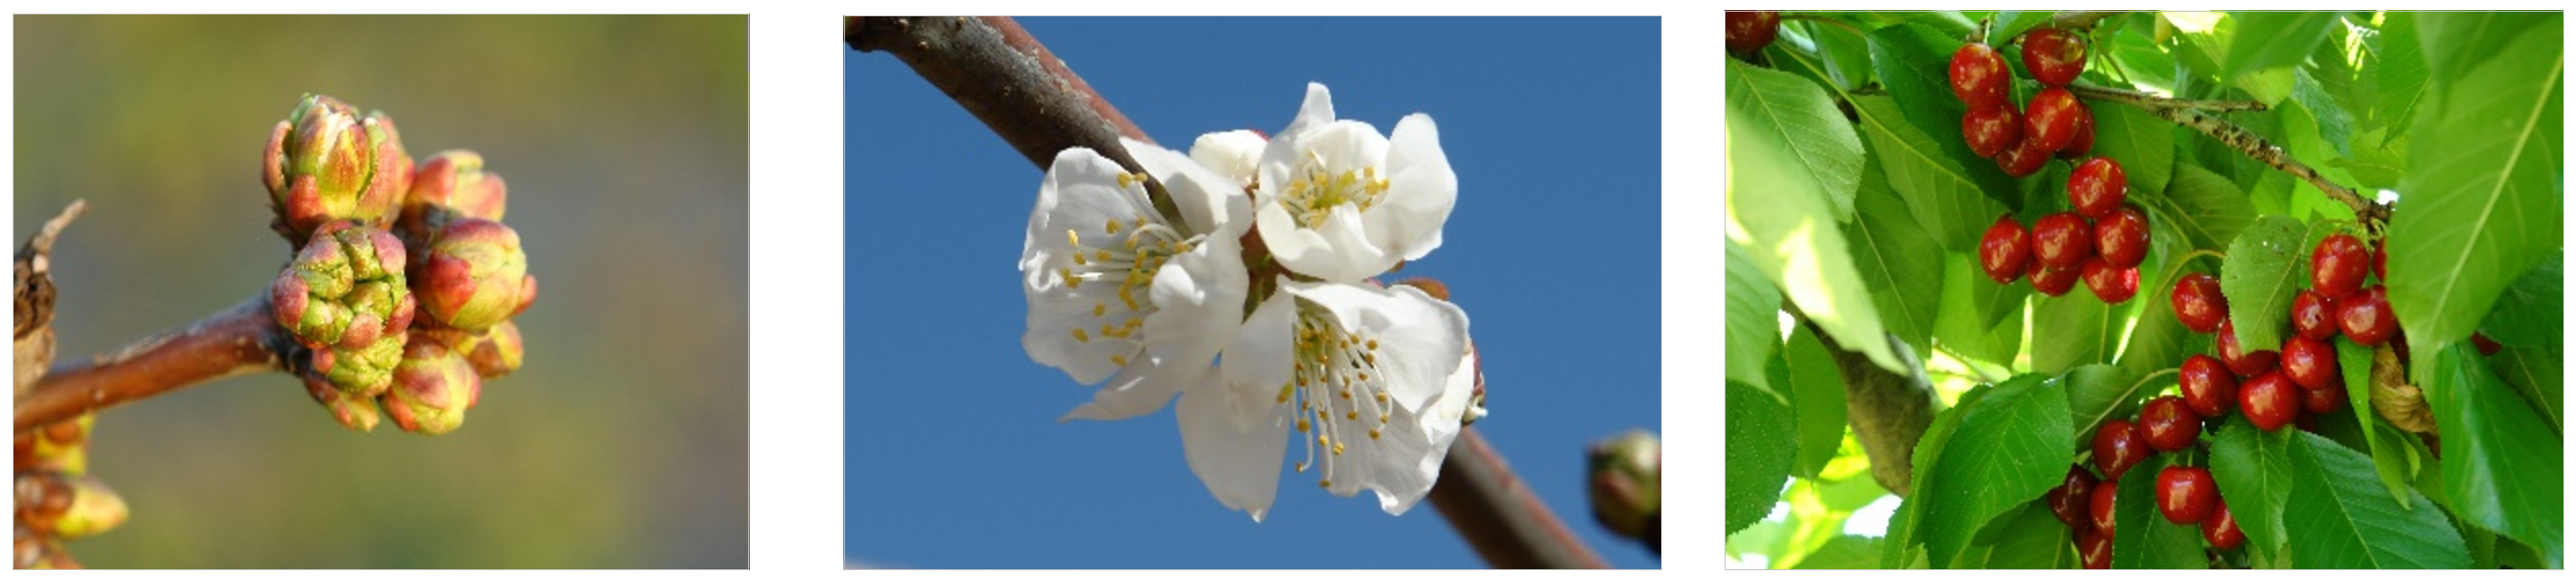
\includegraphics{images/pheno_stages.png}

\begin{itemize}
\tightlist
\item
  \textbf{left image:} BBCH stage 55 (single flower buds visible (still closed), green scales slightly open)
\item
  \textbf{middle image:} BBCH stage 65 (full flowering: at least 50\% of flowers open, first petals falling)
\item
  \textbf{right image:} BBCH stage 89 (fruit ripe for harvesting)
\end{itemize}

\section{Climate change and impact projection}\label{climate-change-and-impact-projection}

Before using \texttt{chillR}, there's a brief overview of climate change, because the upcoming work will mainly focus on predicting how global warming might affect phenology-related metrics.

Climate change refers to long-term changes in temperatures and weather patterns. While these changes can occur naturally --- such as fluctuations in solar activity --- since the 19th century, climate change has primarily been driven by human activities, particularly the burning of fossil fuels like coal, oil, and natural gas.

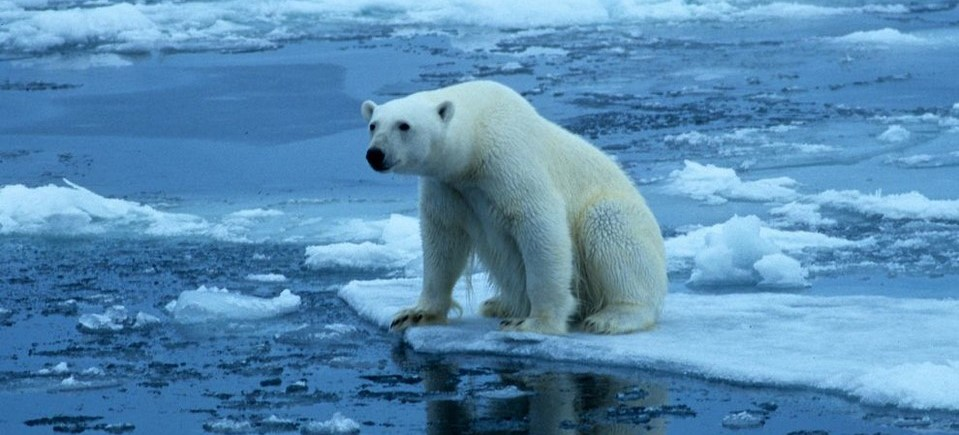
\includegraphics{images/polar-bear-01.jpg}

\subsection{The drivers of climate change}\label{the-drivers-of-climate-change}

To understand what's happening to our planet, it's important to know the main causes of climate change. This helps us spot false claims that things like the sun, cities, or natural changes in the climate are the main reasons for global warming. The truth is simple: human-made greenhouse gas emissions are heating up our planet, and the only way to stop this is to greatly reduce these emissions.

The video below, titled \emph{Climate Change 1 - Drivers of Climate Change}, is the first in a series of four videos on the topic of climate change presented by \href{https://www.gartenbauwissenschaft.uni-bonn.de/author/prof.-dr.-eike-luedeling/}{Eike Lüdeling}. It provides a comprehensive overview of the primary drivers of global climate change, such as greenhouse gases, aerosols, solar radiation, ozone, and others.

\subsection{What's already known}\label{whats-already-known}

The next video, \emph{Climate Change 2 - Recent Warming}, explores climatic changes that have already occurred or for which there is substantial evidence. It demonstrates that the planet has experienced significant warming for several decades, almost globally.

\subsection{Future scenarios}\label{future-scenarios}

When it comes to climate change, the most severe impacts are still ahead. This is largely due to the significantly higher rate of greenhouse gas emissions observed over the past few decades, with no signs of a slowdown in the near future. As a result, the human-induced `forcing' effect on our climate has reached unprecedented levels, making it likely that future changes will occur even more rapidly than those we have already witnessed. The next video \emph{Climate Change 3 - Future scenarios} introduces the methods that climate scientists employ to forecast future conditions and presents climate scenarios developed by these scientists, which researchers in other fields can use to project the impacts of climate change on ecological and agricultural systems.

\subsection{Impact projections approaches}\label{impact-projections-approaches}

Having robust climate scenarios is essential, but they only take us partway toward reliable assessments of climate change impacts. A potentially greater challenge lies in translating these climate scenarios into biological consequences. To achieve this, we need impact models or other methods to derive the impacts of climate change. The last video \emph{Climate change 4 - impact projection approaches} introduces various methods for projecting climate impacts.

\subsection{\texorpdfstring{\texttt{Exercises} on climate change}{Exercises on climate change}}\label{exercises-on-climate-change}

\begin{enumerate}
\def\labelenumi{\arabic{enumi}.}
\tightlist
\item
  \emph{List the main drivers of climate change at the decade to century scale, and briefly explain the mechanism through which the currently most important driver affects our climate.}
\end{enumerate}

The main drivers of climate change on a decade-to-century scale include:

\begin{itemize}
\item
  \textbf{Greenhouse Gases (GHGs):} GHGs like carbon dioxide (CO₂), methane (CH₄), and nitrous oxide (N₂O) trap heat in the atmosphere, leading to the greenhouse effect, which raises Earth's temperature. The increase in these gases is primarily due to human activities, such as burning fossil fuels, industrial processes, and deforestation
\item
  \textbf{Aerosols:} Particles in the atmosphere that can cool the climate by reflecting sunlight. They come from both natural sources (e.g.~sea salt, dust, volcanic eruptions, fires) and human activities (e.g.power plants, cars, fires and cook stove). They are major climate driver in industrial centers (e.g.~China)
\item
  \textbf{Sun:} Solar radiation heats the Earth, with minor fluctuations occurring over time due to cycles in solar activity, such as sunspots. Although these variations contribute only a small portion to the current climate changes, they play a significant role in driving climate change over geological timescales
\item
  \textbf{Ozone:} Ozone in the stratosphere protects Earth from UV-B radiation, while tropospheric ozone acts as a greenhouse gas and contributes to warming
\item
  \textbf{Surface albedo:} The reflectivity of the Earth's surface affects how much solar energy is absorbed. Light surfaces (like ice) reflect more energy, while dark surfaces (like forests or oceans) absorb more, influencing the planet's heat balance. Changes in surface reflectivity, such as melting ice and snow, decrease the albedo effect, leading to more heat absorption and further warming
\end{itemize}

The currently most important driver of climate change is greenhouse gases, particularly CO₂. The mechanism through which CO₂ affects the climate involves the greenhouse effect: CO₂ molecules in the atmosphere absorb long-wave radiation emitted from the Earth's surface and re-radiate it in all directions, including back toward the surface. This process traps heat and increases global temperatures, driving many of the changes we observe in climate patterns.

\begin{enumerate}
\def\labelenumi{\arabic{enumi}.}
\setcounter{enumi}{1}
\tightlist
\item
  \emph{Explain briefly what is special about temperature dynamics of recent decades, and why we have good reasons to be concerned.}
\end{enumerate}

In recent decades, global temperatures have been rising at a faster rate than at any other time in human history. This trend is evident from the fact that the hottest years on record have all occurred within the last few decades. One striking example is the extreme heat in Siberia in the spring of 2020, where temperatures were up to 8°C above the recent average. This trend is particularly concerning because it is mainly driven by human activities, especially the emission of greenhouse gases. Unlike previous climate changes, which took place slowly over long periods, today's fast rise in temperatures increases the risk of triggering dangerous effects, like melting permafrost and losing ice cover, which could make global warming even worse. Even a small increase of 1.5°C could seriously upset the balance of our climate, showing how important it is to take action against these human-caused changes.

\begin{enumerate}
\def\labelenumi{\arabic{enumi}.}
\setcounter{enumi}{2}
\tightlist
\item
  \emph{What does the abbreviation `RCP' stand for, how are RCPs defined, and what is their role in projecting future climates?}
\end{enumerate}

RCP stands for Representative Concentration Pathways, which are essential scenarios used in climate modeling to project potential future greenhouse gas emissions and their impacts on the climate. RCPs are defined by the level of radiative forcing --- measured in watts per square meter (W/m²) --- that is expected by the end of the 21st century. Each pathway corresponds to a specific amount of greenhouse gas concentrations, which can significantly influence global temperatures. The role of RCPs is to serve as inputs for climate models, helping to produce future climate scenarios, which are essential for understanding the potential impacts of climate change and planning appropriate mitigation and adaptation strategies.

\begin{enumerate}
\def\labelenumi{\arabic{enumi}.}
\setcounter{enumi}{3}
\tightlist
\item
  \emph{Briefly describe the 4 climate impact projection methods described in the fourth video.}
\end{enumerate}

The four climate impact projection methods described in the fourth video are:

\begin{itemize}
\item
  \textbf{Statistical models:} These models establish relationships between climate parameters and impact measures, such as crop yield. They use historical data to explain past trends and project future climate impacts. Their primary limitation is that the statistical relationships may not remain valid under future climate conditions, and they may overlook important factors
\item
  \textbf{Species Distribution Modeling:} Also known as ecological niche modeling, this method predicts the future distribution of species by relating current presence or absence data to climatic parameters. However, these models may assume species are in equilibrium with the climate, which is often not the case
\item
  \textbf{Process based models:} These models aim to represent all major system processes using equations, capturing the scientific knowledge of processes like crop growth, phenology or hydrology. However, they are limited by the lack of complete understanding of complex systems, and often require extensive parameterization or assumptions
\item
  \textbf{Climate Analogue models:} This method identifies current locations with climates similar to those expected in the future at another site, offering real-world examples that can guide adaptation strategies. However, they may be limited by differences in non-climatic factors and lack of suitable data, making it difficult to draw clear conditions
\end{itemize}

\section{Winter chill projections}\label{winter-chill-projections}

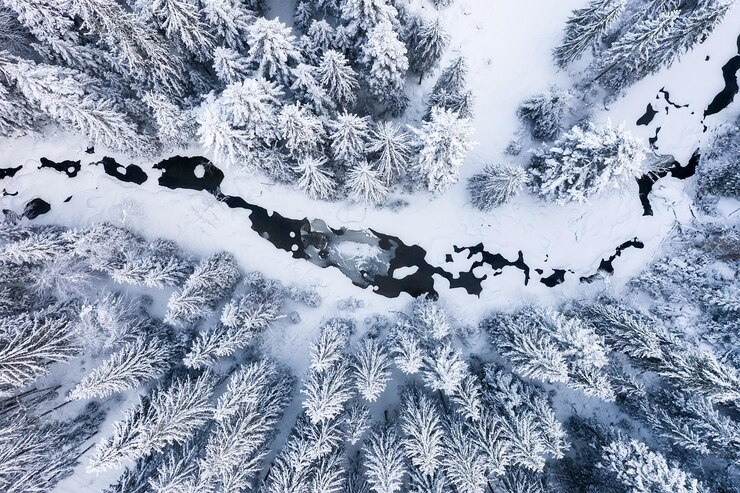
\includegraphics[width=7.8125in,height=\textheight]{images/winter.jpg}

\subsection{Learning goals}\label{learning-goals-2}

\begin{itemize}
\tightlist
\item
  Be aware of past studies that have projected climate change impacts on winter chill
\item
  Get a rough idea of how such studies are done
\item
  Get curious about how to do such studies
\end{itemize}

\subsection{Winter chill projections}\label{winter-chill-projections-1}

This lesson gives an overview about how winter chill can be modeled. More specifically, it introduces various studies that have been conducted on this topic. These studies are explored to illustrate how the methodological components fit together. If everything goes as planned, most of the analyses behind these studies should be achievable by the end of this class.

\subsubsection{Winter chill in Oman}\label{winter-chill-in-oman}

As a student at the University of Kassel, there was an opportunity to participate in research projects centered on mountain oases in the Sultanate of Oman. These systems later became the focus of a PhD project, where the interest in winter chill first emerged. Initially, the study plan was different, aiming to calculate nutrient budgets for the oases, which required measuring the yields of the various fruit trees in these regions. The following provides an impression of the oasis orchards:

\subsection{\texorpdfstring{\texttt{Exercises} on past chill projections}{Exercises on past chill projections}}\label{exercises-on-past-chill-projections}

\begin{enumerate}
\def\labelenumi{\arabic{enumi}.}
\item
  \emph{Sketch out three data access and processing challenges that had to be overcome in order to produce chill projections with state-of-the-art methodology.}
\item
  \emph{Outline, in your understanding, the basic steps that are necessary to make such projections.}
\end{enumerate}

\section{Manual chill}\label{manual-chill}

This chapter explains how to calculate Chilling Hours using R and the \texttt{chillR} package. Chilling Hours measure the number of hours where temperatures are between 0°C and 7.2°C, which is important for certain plants to meet their cold requirements during dormancy and grow properly.

\subsection{Learning goals}\label{learning-goals-3}

\begin{itemize}
\tightlist
\item
  Learn about some basic R operations we need for calculating Chilling Hours
\item
  Be able to calculate Chilling Hours
\item
  Understand what an R function is
\item
  Be able to write your own basic function
\end{itemize}

\subsection{Chilling hours calculation using chillR}\label{chilling-hours-calculation-using-chillr}

Basic models like the Chilling Hours Model are simple and can be calculated manually, especially if familiar with R or spreadsheet software. This example will show how to understand and use the functions in the \texttt{chillR} package to calculate these chill hours.

\subsubsection{\texorpdfstring{\textbf{Data Requirements}}{Data Requirements}}\label{data-requirements}

The Chilling Hours Model is relatively simple but requires hourly temperature data. A common challenge is the unavailability of such data, though approximations can be made from daily records using \texttt{chillR} tools. For this example, a sample dataset, \texttt{Winters\_hours\_gaps}, provided within \texttt{chillR}, was used. It contains hourly temperature data recorded in 2008 from a walnut orchard in Winters, California, and is structured with columns for year, month, day, hour, and temperature.

\subsubsection{Loading and Preparing Data}\label{loading-and-preparing-data}

To work with \texttt{chillR}, the package was loaded using \texttt{library(chillR)}. The data can also be imported via \texttt{read.table()} or \texttt{read.csv()} for external datasets. The \texttt{Winters\_hours\_gaps} dataset was filtered to retain only the essential columns: year, month, day, hour, and temperature. This cleaned version, stored in a new dataframe called \texttt{hourtemps}, ensures the data is in the correct format for calculating Chilling Hours:

\begin{Shaded}
\begin{Highlighting}[]
\NormalTok{hourtemps }\OtherTok{\textless{}{-}}\NormalTok{ Winters\_hours\_gaps[,}\FunctionTok{c}\NormalTok{(}\StringTok{"Year"}\NormalTok{,}
                                   \StringTok{"Month"}\NormalTok{,}
                                   \StringTok{"Day"}\NormalTok{,}
                                   \StringTok{"Hour"}\NormalTok{,}
                                   \StringTok{"Temp"}\NormalTok{)]}
\end{Highlighting}
\end{Shaded}

\begingroup\fontsize{15}{17}\selectfont

\begin{tabu} to \linewidth {>{\centering}X>{\centering}X>{\centering}X>{\centering}X>{\centering}X}
\hline
Year & Month & Day & Hour & Temp\\
\hline
2008 & 3 & 3 & 10 & 15.127\\
\hline
2008 & 3 & 3 & 11 & 17.153\\
\hline
2008 & 3 & 3 & 12 & 18.699\\
\hline
2008 & 3 & 3 & 13 & 18.699\\
\hline
2008 & 3 & 3 & 14 & 18.842\\
\hline
2008 & 3 & 3 & 15 & 19.508\\
\hline
2008 & 3 & 3 & 16 & 19.318\\
\hline
2008 & 3 & 3 & 17 & 17.701\\
\hline
2008 & 3 & 3 & 18 & 15.414\\
\hline
2008 & 3 & 3 & 19 & 12.727\\
\hline
\end{tabu}
\endgroup{}

\subsubsection{\texorpdfstring{\textbf{Manual Calculation of Chilling Hours}}{Manual Calculation of Chilling Hours}}\label{manual-calculation-of-chilling-hours}

Chilling Hours are defined as any hour where the temperature falls between 0°C and 7.2°C. A logical comparison was used in R to identify whether each hour met this criterion:

\begin{Shaded}
\begin{Highlighting}[]
\NormalTok{hourtemps[, }\StringTok{"Chilling\_Hour"}\NormalTok{] }\OtherTok{\textless{}{-}}\NormalTok{ hourtemps}\SpecialCharTok{$}\NormalTok{Temp }\SpecialCharTok{\textgreater{}=} \DecValTok{0} \SpecialCharTok{\&}\NormalTok{ hourtemps}\SpecialCharTok{$}\NormalTok{Temp }\SpecialCharTok{\textless{}=} \FloatTok{7.2}
\end{Highlighting}
\end{Shaded}

\begingroup\fontsize{15}{17}\selectfont

\begin{tabu} to \linewidth {>{\centering}X>{\centering}X>{\centering}X>{\centering}X>{\centering}X>{\centering}X}
\hline
Year & Month & Day & Hour & Temp & Chilling\_Hour\\
\hline
2008 & 3 & 3 & 10 & 15.127 & FALSE\\
\hline
2008 & 3 & 3 & 11 & 17.153 & FALSE\\
\hline
2008 & 3 & 3 & 12 & 18.699 & FALSE\\
\hline
2008 & 3 & 3 & 13 & 18.699 & FALSE\\
\hline
2008 & 3 & 3 & 14 & 18.842 & FALSE\\
\hline
2008 & 3 & 3 & 15 & 19.508 & FALSE\\
\hline
2008 & 3 & 3 & 16 & 19.318 & FALSE\\
\hline
2008 & 3 & 3 & 17 & 17.701 & FALSE\\
\hline
2008 & 3 & 3 & 18 & 15.414 & FALSE\\
\hline
2008 & 3 & 3 & 19 & 12.727 & FALSE\\
\hline
\end{tabu}
\endgroup{}

A new column, \texttt{Chilling\_Hour}, was created, indicating whether a given hour was a valid Chilling Hour (TRUE or FALSE). These values can then be summed to calculate the total number of Chilling Hours for any period using the \texttt{sum()} function.

\subsubsection{Automation with Functions}\label{automation-with-functions}

A function is a tool that automates a particular procedure. It consists of a name, some arguments that are passed to the function, and some code that should be executed. To avoid repeating manual calculations, a reusable function called \texttt{CH} was created to automate the addition of a \texttt{Chilling\_Hour} column:

\begin{Shaded}
\begin{Highlighting}[]
\NormalTok{CH }\OtherTok{\textless{}{-}} \ControlFlowTok{function}\NormalTok{(hourtemps) \{}
\NormalTok{  hourtemps[, }\StringTok{"Chilling\_Hour"}\NormalTok{] }\OtherTok{\textless{}{-}}\NormalTok{ hourtemps}\SpecialCharTok{$}\NormalTok{Temp }\SpecialCharTok{\textgreater{}=} \DecValTok{0} \SpecialCharTok{\&}\NormalTok{ hourtemps}\SpecialCharTok{$}\NormalTok{Temp }\SpecialCharTok{\textless{}=} \FloatTok{7.2}
  \FunctionTok{return}\NormalTok{(hourtemps)}
\NormalTok{\}}
\end{Highlighting}
\end{Shaded}

This function applies to any appropriately structured dataset. Additionally, a more complex function, \texttt{sum\_CH}, was developed to calculate the total Chilling Hours between two specific dates:

\begin{Shaded}
\begin{Highlighting}[]
\NormalTok{sum\_CH }\OtherTok{\textless{}{-}} \ControlFlowTok{function}\NormalTok{(hourtemps, Start\_Year,}
\NormalTok{                              Start\_Month,}
\NormalTok{                              Start\_Day, }
\NormalTok{                              Start\_Hour, }
\NormalTok{                              End\_Year, }
\NormalTok{                              End\_Month, }
\NormalTok{                              End\_Day, }
\NormalTok{                              End\_Hour) }
  
\NormalTok{\{hourtemps[,}\StringTok{"Chilling\_Hour"}\NormalTok{] }\OtherTok{\textless{}{-}}\NormalTok{ hourtemps}\SpecialCharTok{$}\NormalTok{Temp }\SpecialCharTok{\textgreater{}} \DecValTok{0} \SpecialCharTok{\&}
\NormalTok{                                hourtemps}\SpecialCharTok{$}\NormalTok{Temp  }\SpecialCharTok{\textless{}=} \FloatTok{7.2}

\NormalTok{  Start\_Date }\OtherTok{\textless{}{-}} \FunctionTok{which}\NormalTok{(hourtemps}\SpecialCharTok{$}\NormalTok{Year }\SpecialCharTok{==}\NormalTok{ Start\_Year }\SpecialCharTok{\&} 
\NormalTok{                      hourtemps}\SpecialCharTok{$}\NormalTok{Month }\SpecialCharTok{==}\NormalTok{ Start\_Month }\SpecialCharTok{\&}
\NormalTok{                      hourtemps}\SpecialCharTok{$}\NormalTok{Day }\SpecialCharTok{==}\NormalTok{ Start\_Day }\SpecialCharTok{\&}
\NormalTok{                      hourtemps}\SpecialCharTok{$}\NormalTok{Hour }\SpecialCharTok{==}\NormalTok{ Start\_Hour)}
  
\NormalTok{  End\_Date }\OtherTok{\textless{}{-}} \FunctionTok{which}\NormalTok{(hourtemps}\SpecialCharTok{$}\NormalTok{Year }\SpecialCharTok{==}\NormalTok{ End\_Year }\SpecialCharTok{\&}
\NormalTok{                    hourtemps}\SpecialCharTok{$}\NormalTok{Month }\SpecialCharTok{==}\NormalTok{ End\_Month }\SpecialCharTok{\&}
\NormalTok{                    hourtemps}\SpecialCharTok{$}\NormalTok{Day }\SpecialCharTok{==}\NormalTok{ End\_Day }\SpecialCharTok{\&} 
\NormalTok{                    hourtemps}\SpecialCharTok{$}\NormalTok{Hour }\SpecialCharTok{==}\NormalTok{ End\_Hour)}
  
\NormalTok{  CHs }\OtherTok{\textless{}{-}} \FunctionTok{sum}\NormalTok{(hourtemps}\SpecialCharTok{$}\NormalTok{Chilling\_Hour[Start\_Date}\SpecialCharTok{:}\NormalTok{End\_Date])}
  \FunctionTok{return}\NormalTok{(CHs)}
\NormalTok{\}}
\end{Highlighting}
\end{Shaded}

This function calculates Chilling Hours for a user-defined date range, using the \texttt{which()} function to identify the relevant rows in the dataset corresponding to the start and end dates.

To simplify the parameter passing, compact strings in the format \texttt{YEARMODAHO} (year, month, day, and hour as consecutive numbers) can be used instead of individual parameters for year, month, day, and hour. The start and end times are now passed as strings, from which the required values are extracted using the \texttt{substr()} function and converted to numeric values with \texttt{as.numeric()}.

\begin{Shaded}
\begin{Highlighting}[]
\NormalTok{sum\_CH }\OtherTok{\textless{}{-}} \ControlFlowTok{function}\NormalTok{(hourtemps, }
\NormalTok{                   startYEARMODAHO,}
\NormalTok{                   endYEARMODAHO)}
\NormalTok{\{hourtemps[,}\StringTok{"Chilling\_Hour"}\NormalTok{] }\OtherTok{\textless{}{-}}\NormalTok{ hourtemps}\SpecialCharTok{$}\NormalTok{Temp }\SpecialCharTok{\textgreater{}} \DecValTok{0} \SpecialCharTok{\&}
\NormalTok{  hourtemps}\SpecialCharTok{$}\NormalTok{Temp }\SpecialCharTok{\textless{}=} \FloatTok{7.2}

\NormalTok{startYear }\OtherTok{\textless{}{-}} \FunctionTok{as.numeric}\NormalTok{(}\FunctionTok{substr}\NormalTok{(startYEARMODAHO, }\DecValTok{1}\NormalTok{, }\DecValTok{4}\NormalTok{))}
\NormalTok{startMonth }\OtherTok{\textless{}{-}} \FunctionTok{as.numeric}\NormalTok{(}\FunctionTok{substr}\NormalTok{(startYEARMODAHO, }\DecValTok{5}\NormalTok{, }\DecValTok{6}\NormalTok{))}
\NormalTok{startDay }\OtherTok{\textless{}{-}} \FunctionTok{as.numeric}\NormalTok{(}\FunctionTok{substr}\NormalTok{(startYEARMODAHO, }\DecValTok{7}\NormalTok{, }\DecValTok{8}\NormalTok{))}
\NormalTok{startHour }\OtherTok{\textless{}{-}} \FunctionTok{as.numeric}\NormalTok{(}\FunctionTok{substr}\NormalTok{(startYEARMODAHO, }\DecValTok{9}\NormalTok{, }\DecValTok{10}\NormalTok{))}

\NormalTok{endYear }\OtherTok{\textless{}{-}} \FunctionTok{as.numeric}\NormalTok{(}\FunctionTok{substr}\NormalTok{(endYEARMODAHO, }\DecValTok{1}\NormalTok{, }\DecValTok{4}\NormalTok{))}
\NormalTok{endMonth }\OtherTok{\textless{}{-}} \FunctionTok{as.numeric}\NormalTok{(}\FunctionTok{substr}\NormalTok{(endYEARMODAHO, }\DecValTok{5}\NormalTok{, }\DecValTok{6}\NormalTok{))}
\NormalTok{endDay }\OtherTok{\textless{}{-}} \FunctionTok{as.numeric}\NormalTok{(}\FunctionTok{substr}\NormalTok{(endYEARMODAHO, }\DecValTok{7}\NormalTok{, }\DecValTok{8}\NormalTok{))}
\NormalTok{endHour }\OtherTok{\textless{}{-}} \FunctionTok{as.numeric}\NormalTok{(}\FunctionTok{substr}\NormalTok{(endYEARMODAHO, }\DecValTok{9}\NormalTok{, }\DecValTok{10}\NormalTok{))}


\NormalTok{Start\_row }\OtherTok{\textless{}{-}} \FunctionTok{which}\NormalTok{(hourtemps}\SpecialCharTok{$}\NormalTok{Year }\SpecialCharTok{==}\NormalTok{ startYear }\SpecialCharTok{\&}
\NormalTok{                   hourtemps}\SpecialCharTok{$}\NormalTok{Month }\SpecialCharTok{==}\NormalTok{ startMonth }\SpecialCharTok{\&}
\NormalTok{                   hourtemps}\SpecialCharTok{$}\NormalTok{Day }\SpecialCharTok{==}\NormalTok{ startDay }\SpecialCharTok{\&}
\NormalTok{                   hourtemps}\SpecialCharTok{$}\NormalTok{Hour }\SpecialCharTok{==}\NormalTok{ startHour}
\NormalTok{)}
\NormalTok{End\_row }\OtherTok{\textless{}{-}} \FunctionTok{which}\NormalTok{(hourtemps}\SpecialCharTok{$}\NormalTok{Year }\SpecialCharTok{==}\NormalTok{ endYear }\SpecialCharTok{\&}
\NormalTok{                 hourtemps}\SpecialCharTok{$}\NormalTok{Month }\SpecialCharTok{==}\NormalTok{ endMonth }\SpecialCharTok{\&}
\NormalTok{                 hourtemps}\SpecialCharTok{$}\NormalTok{Day }\SpecialCharTok{==}\NormalTok{ endDay }\SpecialCharTok{\&}
\NormalTok{                 hourtemps}\SpecialCharTok{$}\NormalTok{Hour }\SpecialCharTok{==}\NormalTok{ endHour}
\NormalTok{)}

\NormalTok{CHs }\OtherTok{\textless{}{-}} \FunctionTok{sum}\NormalTok{(hourtemps}\SpecialCharTok{$}\NormalTok{Chilling\_Hour[Start\_row}\SpecialCharTok{:}\NormalTok{End\_row])}
\FunctionTok{return}\NormalTok{(CHs)}

\NormalTok{\}}
\end{Highlighting}
\end{Shaded}

\subsubsection{Application Example}\label{application-example}

The functions created allow for efficient calculation of Chilling Hours. For instance, using the \texttt{sum\_CH()} function, it was calculated that between April 1st and October 11th, 2008, the walnut orchard experienced 77 Chilling Hours:

\begin{Shaded}
\begin{Highlighting}[]
\FunctionTok{sum\_CH}\NormalTok{(hourtemps, }\AttributeTok{startYEARMODAHO =}\DecValTok{2008040100}\NormalTok{,}
                  \AttributeTok{endYEARMODAHO =} \DecValTok{2008101100}\NormalTok{)}
\end{Highlighting}
\end{Shaded}

\begin{verbatim}
## [1] 77
\end{verbatim}

\subsection{\texorpdfstring{\texttt{Exercises} on basic chill modeling}{Exercises on basic chill modeling}}\label{exercises-on-basic-chill-modeling}

\begin{enumerate}
\def\labelenumi{\arabic{enumi}.}
\tightlist
\item
  \emph{Write a basic function that calculates warm hours (\textgreater25°C).}
\end{enumerate}

\begin{Shaded}
\begin{Highlighting}[]
\NormalTok{WH }\OtherTok{\textless{}{-}} \ControlFlowTok{function}\NormalTok{(data)}
\NormalTok{  \{data[, }\StringTok{"Warm\_Hour"}\NormalTok{] }\OtherTok{\textless{}{-}}\NormalTok{ data}\SpecialCharTok{$}\NormalTok{Temp }\SpecialCharTok{\textgreater{}} \DecValTok{25}
  \FunctionTok{return}\NormalTok{(data)}
\NormalTok{\}}
\end{Highlighting}
\end{Shaded}

\begin{enumerate}
\def\labelenumi{\arabic{enumi}.}
\setcounter{enumi}{1}
\tightlist
\item
  \emph{Apply this function to the} \texttt{Winters\_hours\_gaps} \emph{dataset.}
\end{enumerate}

\begin{Shaded}
\begin{Highlighting}[]
\FunctionTok{WH}\NormalTok{(Winters\_hours\_gaps)}
\end{Highlighting}
\end{Shaded}

\begingroup\fontsize{15}{17}\selectfont

\begin{tabu} to \linewidth {>{\centering}X>{\centering}X>{\centering}X>{\centering}X>{\centering}X>{\centering}X>{\centering}X}
\hline
Year & Month & Day & Hour & Temp\_gaps & Temp & Warm\_Hour\\
\hline
2008 & 3 & 3 & 10 & 15.127 & 15.127 & FALSE\\
\hline
2008 & 3 & 3 & 11 & 17.153 & 17.153 & FALSE\\
\hline
2008 & 3 & 3 & 12 & 18.699 & 18.699 & FALSE\\
\hline
2008 & 3 & 3 & 13 & 18.699 & 18.699 & FALSE\\
\hline
2008 & 3 & 3 & 14 & 18.842 & 18.842 & FALSE\\
\hline
2008 & 3 & 3 & 15 & 19.508 & 19.508 & FALSE\\
\hline
2008 & 3 & 3 & 16 & 19.318 & 19.318 & FALSE\\
\hline
2008 & 3 & 3 & 17 & 17.701 & 17.701 & FALSE\\
\hline
2008 & 3 & 3 & 18 & 15.414 & 15.414 & FALSE\\
\hline
2008 & 3 & 3 & 19 & 12.727 & 12.727 & FALSE\\
\hline
\end{tabu}
\endgroup{}

\begin{enumerate}
\def\labelenumi{\arabic{enumi}.}
\setcounter{enumi}{2}
\tightlist
\item
  \emph{Extend this function, so that it can take start and end dates as inputs and sums up warm hours between these dates.}
\end{enumerate}

\begin{Shaded}
\begin{Highlighting}[]
\NormalTok{sum\_WH }\OtherTok{\textless{}{-}} \ControlFlowTok{function}\NormalTok{(data, }
\NormalTok{                   startYEARMODAHO,}
\NormalTok{                   endYEARMODAHO)}
  
\NormalTok{\{data[,}\StringTok{"Warm\_Hour"}\NormalTok{] }\OtherTok{\textless{}{-}}\NormalTok{ data}\SpecialCharTok{$}\NormalTok{Temp }\SpecialCharTok{\textgreater{}} \DecValTok{25}

\NormalTok{startYear }\OtherTok{\textless{}{-}} \FunctionTok{as.numeric}\NormalTok{(}\FunctionTok{substr}\NormalTok{(startYEARMODAHO, }\DecValTok{1}\NormalTok{, }\DecValTok{4}\NormalTok{))}
\NormalTok{startMonth }\OtherTok{\textless{}{-}} \FunctionTok{as.numeric}\NormalTok{(}\FunctionTok{substr}\NormalTok{(startYEARMODAHO, }\DecValTok{5}\NormalTok{, }\DecValTok{6}\NormalTok{))}
\NormalTok{startDay }\OtherTok{\textless{}{-}} \FunctionTok{as.numeric}\NormalTok{(}\FunctionTok{substr}\NormalTok{(startYEARMODAHO, }\DecValTok{7}\NormalTok{, }\DecValTok{8}\NormalTok{))}
\NormalTok{startHour }\OtherTok{\textless{}{-}} \FunctionTok{as.numeric}\NormalTok{(}\FunctionTok{substr}\NormalTok{(startYEARMODAHO, }\DecValTok{9}\NormalTok{, }\DecValTok{10}\NormalTok{))}

\NormalTok{endYear }\OtherTok{\textless{}{-}} \FunctionTok{as.numeric}\NormalTok{(}\FunctionTok{substr}\NormalTok{(endYEARMODAHO, }\DecValTok{1}\NormalTok{, }\DecValTok{4}\NormalTok{))}
\NormalTok{endMonth }\OtherTok{\textless{}{-}} \FunctionTok{as.numeric}\NormalTok{(}\FunctionTok{substr}\NormalTok{(endYEARMODAHO, }\DecValTok{5}\NormalTok{, }\DecValTok{6}\NormalTok{))}
\NormalTok{endDay }\OtherTok{\textless{}{-}} \FunctionTok{as.numeric}\NormalTok{(}\FunctionTok{substr}\NormalTok{(endYEARMODAHO, }\DecValTok{7}\NormalTok{, }\DecValTok{8}\NormalTok{))}
\NormalTok{endHour }\OtherTok{\textless{}{-}} \FunctionTok{as.numeric}\NormalTok{(}\FunctionTok{substr}\NormalTok{(endYEARMODAHO, }\DecValTok{9}\NormalTok{, }\DecValTok{10}\NormalTok{))}


\NormalTok{Start\_Date }\OtherTok{\textless{}{-}} \FunctionTok{which}\NormalTok{(data}\SpecialCharTok{$}\NormalTok{Year }\SpecialCharTok{==}\NormalTok{ startYear }\SpecialCharTok{\&}
\NormalTok{                    data}\SpecialCharTok{$}\NormalTok{Month }\SpecialCharTok{==}\NormalTok{ startMonth }\SpecialCharTok{\&}
\NormalTok{                    data}\SpecialCharTok{$}\NormalTok{Day }\SpecialCharTok{==}\NormalTok{ startDay }\SpecialCharTok{\&}
\NormalTok{                    data}\SpecialCharTok{$}\NormalTok{Hour }\SpecialCharTok{==}\NormalTok{ startHour)}

\NormalTok{End\_Date }\OtherTok{\textless{}{-}} \FunctionTok{which}\NormalTok{(data}\SpecialCharTok{$}\NormalTok{Year }\SpecialCharTok{==}\NormalTok{ endYear }\SpecialCharTok{\&}
\NormalTok{                  data}\SpecialCharTok{$}\NormalTok{Month }\SpecialCharTok{==}\NormalTok{ endMonth }\SpecialCharTok{\&}
\NormalTok{                  data}\SpecialCharTok{$}\NormalTok{Day }\SpecialCharTok{==}\NormalTok{ endDay }\SpecialCharTok{\&}
\NormalTok{                  data}\SpecialCharTok{$}\NormalTok{Hour }\SpecialCharTok{==}\NormalTok{ endHour)}

\NormalTok{WHs }\OtherTok{\textless{}{-}} \FunctionTok{sum}\NormalTok{(data}\SpecialCharTok{$}\NormalTok{Warm\_Hour[Start\_Date}\SpecialCharTok{:}\NormalTok{End\_Date])}
\FunctionTok{return}\NormalTok{(WHs)}
\NormalTok{\}}
\end{Highlighting}
\end{Shaded}

\begin{Shaded}
\begin{Highlighting}[]
\FunctionTok{sum\_WH}\NormalTok{(Winters\_hours\_gaps, }\AttributeTok{startYEARMODAHO =} \DecValTok{2008080100}\NormalTok{, }
                           \AttributeTok{endYEARMODAHO =} \DecValTok{2008083100}\NormalTok{)}
\end{Highlighting}
\end{Shaded}

\begin{verbatim}
## [1] 283
\end{verbatim}

During the month of August 2008, from the 1st to the 31st, the walnut orchard experienced a total of 283 warm hours (defined as hours when the temperature exceeded 25°C).

\section{Chill}\label{chill}

In this chapter, various chill models will be explored using the \texttt{chillR} package in R, which simplifies the calculation of chilling hours and other dormancy-related metrics based on temperature data.

\subsection{Learning goals}\label{learning-goals-4}

\begin{itemize}
\tightlist
\item
  Learn how to run chill models using \texttt{chillR}
\item
  Learn how to produce your own temperature response model in \texttt{chillR}
\end{itemize}

\subsection{\texorpdfstring{\texttt{Chilling\_Hours()} function}{Chilling\_Hours() function}}\label{chilling_hours-function}

The \texttt{Chilling\_Hours()} function calculates the time during which temperatures fall within a key range for chill accumulation. It takes hourly temperature data as input and, by default, provides the cumulative amount of chilling accumulated over time.

\begin{Shaded}
\begin{Highlighting}[]
\FunctionTok{Chilling\_Hours}\NormalTok{(Winters\_hours\_gaps}\SpecialCharTok{$}\NormalTok{Temp)[}\DecValTok{1}\SpecialCharTok{:}\DecValTok{100}\NormalTok{]}
\end{Highlighting}
\end{Shaded}

\begin{verbatim}
##   [1]  0  0  0  0  0  0  0  0  0  0  0  0  0  0  1  2  2  2  3  4  5  6  6  6  6
##  [26]  6  6  6  6  6  6  6  6  6  6  6  6  6  6  6  6  6  6  6  6  6  6  6  6  6
##  [51]  6  6  6  6  6  6  6  6  6  6  6  7  8  9 10 11 12 13 14 15 16 16 16 16 16
##  [76] 16 16 16 16 16 16 16 16 16 16 17 18 19 20 21 22 23 24 25 25 25 25 25 25 25
\end{verbatim}

The result will show the first 100 values, where the cumulative chilling hours increase as the temperature falls within the specified range.

\subsection{Utah Model}\label{utah-model}

The Utah Model assigns different weights to various temperature ranges, reflecting their impact on chill accumulation. The \texttt{Utah\_Model()} function in \texttt{chillR} calculates these weighted chilling contributions for each hour of temperature data. The output will show the Utah model values for the first 100 hours, where positive, zero, and negative weights are applied based on the temperature:

\begin{Shaded}
\begin{Highlighting}[]
\FunctionTok{Utah\_Model}\NormalTok{(Winters\_hours\_gaps}\SpecialCharTok{$}\NormalTok{Temp)[}\DecValTok{1}\SpecialCharTok{:}\DecValTok{100}\NormalTok{]}
\end{Highlighting}
\end{Shaded}

\begin{verbatim}
##   [1]  0.0 -0.5 -1.5 -2.5 -3.5 -4.5 -5.5 -6.0 -6.0 -6.0 -5.5 -5.0 -4.0 -3.0 -2.0
##  [16] -1.0  0.0  0.5  1.5  2.5  3.5  4.5  5.0  5.0  5.0  4.0  3.0  2.0  1.0  0.0
##  [31] -1.0 -2.0 -2.5 -2.5 -2.0 -1.5 -1.0 -0.5  0.5  1.0  1.5  2.0  2.0  2.5  3.0
##  [46]  3.5  4.0  4.0  4.0  3.5  2.5  1.5  0.5 -0.5 -1.5 -2.5 -3.0 -3.0 -2.5 -1.5
##  [61] -0.5  0.5  1.5  2.5  3.5  4.5  5.5  6.5  7.5  8.5  9.5 10.0 10.0  9.5  9.0
##  [76]  8.5  8.0  7.5  7.0  6.5  6.5  7.0  7.5  8.5  9.5 10.5 11.5 12.5 13.5 14.5
##  [91] 15.5 16.5 17.5 18.5 19.0 19.0 19.0 18.5 17.5 16.5
\end{verbatim}

\subsection{\texorpdfstring{Creating Custom Chill Models with \texttt{step\_model()}}{Creating Custom Chill Models with step\_model()}}\label{creating-custom-chill-models-with-step_model}

The \texttt{step\_model()} function, part of the \texttt{chillR} package, enables the creation of custom chill models based on temperature thresholds and weights. This process involves defining a data frame that specifies temperature ranges and their corresponding weights. Here's an example of a data frame that defines temperature ranges and their corresponding weights:

\begin{Shaded}
\begin{Highlighting}[]
\NormalTok{df }\OtherTok{\textless{}{-}} \FunctionTok{data.frame}\NormalTok{(}
  \AttributeTok{lower =} \FunctionTok{c}\NormalTok{(}\SpecialCharTok{{-}}\DecValTok{1000}\NormalTok{, }\DecValTok{1}\NormalTok{, }\DecValTok{2}\NormalTok{, }\DecValTok{3}\NormalTok{, }\DecValTok{4}\NormalTok{, }\DecValTok{5}\NormalTok{,    }\DecValTok{6}\NormalTok{),}
  \AttributeTok{upper =} \FunctionTok{c}\NormalTok{(    }\DecValTok{1}\NormalTok{, }\DecValTok{2}\NormalTok{, }\DecValTok{3}\NormalTok{, }\DecValTok{4}\NormalTok{, }\DecValTok{5}\NormalTok{, }\DecValTok{6}\NormalTok{, }\DecValTok{1000}\NormalTok{),}
  \AttributeTok{weight =} \FunctionTok{c}\NormalTok{(    }\DecValTok{0}\NormalTok{, }\DecValTok{1}\NormalTok{, }\DecValTok{2}\NormalTok{, }\DecValTok{3}\NormalTok{, }\DecValTok{2}\NormalTok{, }\DecValTok{1}\NormalTok{,    }\DecValTok{0}\NormalTok{))}
\end{Highlighting}
\end{Shaded}

\begingroup\fontsize{15}{17}\selectfont

\begin{tabu} to \linewidth {>{\centering}X>{\centering}X>{\centering}X}
\hline
lower & upper & weight\\
\hline
-1000 & 1 & 0\\
\hline
1 & 2 & 1\\
\hline
2 & 3 & 2\\
\hline
3 & 4 & 3\\
\hline
4 & 5 & 2\\
\hline
5 & 6 & 1\\
\hline
6 & 1000 & 0\\
\hline
\end{tabu}
\endgroup{}

A function called \texttt{custom()} implements a chill model based on this data frame. This function is then applied to the \texttt{Winters\_hours\_gaps} dataset to calculate the chilling contributions:

\begin{Shaded}
\begin{Highlighting}[]
\NormalTok{custom }\OtherTok{\textless{}{-}} \ControlFlowTok{function}\NormalTok{(x) }\FunctionTok{step\_model}\NormalTok{(x, df)}
\FunctionTok{custom}\NormalTok{(Winters\_hours\_gaps}\SpecialCharTok{$}\NormalTok{Temp)[}\DecValTok{1}\SpecialCharTok{:}\DecValTok{100}\NormalTok{]}
\end{Highlighting}
\end{Shaded}

\begin{verbatim}
##   [1]  0  0  0  0  0  0  0  0  0  0  0  0  0  0  0  0  0  0  0  1  4  7  7  7  7
##  [26]  7  7  7  7  7  7  7  7  7  7  7  7  7  7  7  7  7  7  7  7  7  7  7  7  7
##  [51]  7  7  7  7  7  7  7  7  7  7  7  7  7  7  8 10 13 16 19 22 22 22 22 22 22
##  [76] 22 22 22 22 22 22 22 22 22 22 22 22 23 25 27 29 31 34 37 37 37 37 37 37 37
\end{verbatim}

\subsection{Dynamic model}\label{dynamic-model}

The Dynamic Model provides a more complex and reliable approach to calculating chill, with the \texttt{Dynamic\_Model()} function handling the intricate equations involved. This function can be easily applied to the \texttt{Winters\_hours\_gaps} dataset, producing output that displays dynamic chill values for the first 100 hours, reflecting the underlying physiological processes:

\begin{Shaded}
\begin{Highlighting}[]
\FunctionTok{Dynamic\_Model}\NormalTok{(Winters\_hours\_gaps}\SpecialCharTok{$}\NormalTok{Temp)[}\DecValTok{1}\SpecialCharTok{:}\DecValTok{100}\NormalTok{]}
\end{Highlighting}
\end{Shaded}

\begin{verbatim}
##   [1] 0.0000000 0.0000000 0.0000000 0.0000000 0.0000000 0.0000000 0.0000000
##   [8] 0.0000000 0.0000000 0.0000000 0.0000000 0.0000000 0.0000000 0.0000000
##  [15] 0.0000000 0.0000000 0.0000000 0.0000000 0.0000000 0.0000000 0.0000000
##  [22] 0.0000000 0.0000000 0.0000000 0.0000000 0.0000000 0.0000000 0.0000000
##  [29] 0.0000000 0.0000000 0.0000000 0.0000000 0.0000000 0.0000000 0.0000000
##  [36] 0.0000000 0.0000000 0.0000000 0.0000000 0.0000000 0.0000000 0.0000000
##  [43] 0.0000000 0.0000000 0.0000000 0.0000000 0.0000000 0.0000000 0.0000000
##  [50] 0.0000000 0.0000000 0.0000000 0.0000000 0.0000000 0.0000000 0.0000000
##  [57] 0.0000000 0.0000000 0.0000000 0.0000000 0.0000000 0.0000000 0.0000000
##  [64] 0.0000000 0.0000000 0.0000000 0.0000000 0.0000000 0.0000000 0.0000000
##  [71] 0.0000000 0.9698435 0.9698435 0.9698435 0.9698435 0.9698435 0.9698435
##  [78] 0.9698435 0.9698435 0.9698435 0.9698435 0.9698435 0.9698435 0.9698435
##  [85] 0.9698435 0.9698435 0.9698435 0.9698435 0.9698435 0.9698435 0.9698435
##  [92] 0.9698435 0.9698435 0.9698435 0.9698435 0.9698435 0.9698435 0.9698435
##  [99] 0.9698435 0.9698435
\end{verbatim}

\subsection{\texorpdfstring{\texttt{Chilling} and \texttt{tempResponse} functions}{Chilling and tempResponse functions}}\label{chilling-and-tempresponse-functions}

The \texttt{chillR} package offers several functions for analyzing hourly temperature data, including wrapper functions that enable the computation of chill between specific start and end dates. The \texttt{chilling()} function automatically calculates various basic metrics, including Chilling Hours, Utah Model, Dynamic Model, and Growing Degree Hours. It is important to use the \texttt{make\_JDay()} function to add Julian dates (which count the days of the year) to the dataset, ensuring proper functionality.

\begin{Shaded}
\begin{Highlighting}[]
\NormalTok{output }\OtherTok{\textless{}{-}} \FunctionTok{chilling}\NormalTok{(}\FunctionTok{make\_JDay}\NormalTok{(Winters\_hours\_gaps), }\AttributeTok{Start\_JDay =} \DecValTok{90}\NormalTok{, }\AttributeTok{End\_JDay =} \DecValTok{100}\NormalTok{)}
\end{Highlighting}
\end{Shaded}

\begingroup\fontsize{15}{17}\selectfont

\begin{tabu} to \linewidth {>{\centering}X>{\centering}X>{\centering}X>{\centering}X>{\centering}X>{\centering}X>{\centering}X>{\centering}X>{\centering}X}
\hline
Season & End\_year & Season\_days & Data\_days & Perc\_complete & Chilling\_Hours & Utah\_Model & Chill\_portions & GDH\\
\hline
2007/2008 & 2008 & 11 & 11 & 100 & 40 & 15.5 & 2.009147 & 2406.52\\
\hline
\end{tabu}
\endgroup{}

However, there may be instances where not all metrics are desired, or there is a need for different metrics altogether. In such cases, the \texttt{tempResponse} function can be employed. This function is similar to \texttt{chilling()} but offers the flexibility to take a list of specific temperature models to be computed as input.

\begin{Shaded}
\begin{Highlighting}[]
\NormalTok{output }\OtherTok{\textless{}{-}} \FunctionTok{tempResponse}\NormalTok{(}\FunctionTok{make\_JDay}\NormalTok{(Winters\_hours\_gaps), }
                       \AttributeTok{Start\_JDay =} \DecValTok{90}\NormalTok{, }
                       \AttributeTok{End\_JDay =} \DecValTok{100}\NormalTok{, }
                       \AttributeTok{models =} \FunctionTok{list}\NormalTok{(}\AttributeTok{Chill\_Portions =}\NormalTok{ Dynamic\_Model, }\AttributeTok{GDH =}\NormalTok{ GDH))}
\end{Highlighting}
\end{Shaded}

\begingroup\fontsize{15}{17}\selectfont

\begin{tabu} to \linewidth {>{\centering}X>{\centering}X>{\centering}X>{\centering}X>{\centering}X>{\centering}X>{\centering}X}
\hline
Season & End\_year & Season\_days & Data\_days & Perc\_complete & Chill\_Portions & GDH\\
\hline
\cellcolor{gray!10}{2007/2008} & \cellcolor{gray!10}{2008} & \cellcolor{gray!10}{11} & \cellcolor{gray!10}{11} & \cellcolor{gray!10}{100} & \cellcolor{gray!10}{2.009147} & \cellcolor{gray!10}{2406.52}\\
\hline
\end{tabu}
\endgroup{}

This will return only the Dynamic Model and Growing Degree Hours (GDH\textbf{)} values for the specified period.

\subsection{\texorpdfstring{\texttt{Exercises} on chill models}{Exercises on chill models}}\label{exercises-on-chill-models}

\begin{enumerate}
\def\labelenumi{\arabic{enumi}.}
\tightlist
\item
  \emph{Run the} \texttt{chilling()} \emph{function on the} \texttt{Winters\_hours\_gap} \emph{dataset}
\end{enumerate}

\begin{Shaded}
\begin{Highlighting}[]
\NormalTok{august }\OtherTok{\textless{}{-}} \FunctionTok{chilling}\NormalTok{(}\FunctionTok{make\_JDay}\NormalTok{(Winters\_hours\_gaps), }\AttributeTok{Start\_JDay =} \DecValTok{214}\NormalTok{, }\AttributeTok{End\_JDay =} \DecValTok{244}\NormalTok{)}
\end{Highlighting}
\end{Shaded}

\begin{table}
\centering\begingroup\fontsize{15}{17}\selectfont

\begin{tabular}{c|c|c|c|c|c|c|c|c}
\hline
Season & End\_year & Season\_days & Data\_days & Perc\_complete & Chilling\_Hours & Utah\_Model & Chill\_portions & GDH\\
\hline
\cellcolor{gray!10}{2007/2008} & \cellcolor{gray!10}{2008} & \cellcolor{gray!10}{31} & \cellcolor{gray!10}{31} & \cellcolor{gray!10}{100} & \cellcolor{gray!10}{0} & \cellcolor{gray!10}{-569.5} & \cellcolor{gray!10}{0} & \cellcolor{gray!10}{9933.327}\\
\hline
\end{tabular}
\endgroup{}
\end{table}

\begin{enumerate}
\def\labelenumi{\arabic{enumi}.}
\setcounter{enumi}{1}
\tightlist
\item
  \emph{Create your own temperature-weighting chill model using the} \texttt{step\_model()} \emph{function}
\end{enumerate}

\begin{Shaded}
\begin{Highlighting}[]
\NormalTok{df }\OtherTok{\textless{}{-}} \FunctionTok{data.frame}\NormalTok{(}
  \AttributeTok{lower =} \FunctionTok{c}\NormalTok{(}\SpecialCharTok{{-}}\DecValTok{1000}\NormalTok{, }\DecValTok{0}\NormalTok{, }\DecValTok{5}\NormalTok{, }\DecValTok{10}\NormalTok{, }\DecValTok{15}\NormalTok{, }\DecValTok{20}\NormalTok{, }\DecValTok{25}\NormalTok{),  }
  \AttributeTok{upper =} \FunctionTok{c}\NormalTok{(}\DecValTok{0}\NormalTok{, }\DecValTok{5}\NormalTok{, }\DecValTok{10}\NormalTok{, }\DecValTok{15}\NormalTok{, }\DecValTok{20}\NormalTok{, }\DecValTok{25}\NormalTok{, }\DecValTok{1000}\NormalTok{), }
  \AttributeTok{weight =} \FunctionTok{c}\NormalTok{(}\DecValTok{0}\NormalTok{, }\DecValTok{1}\NormalTok{, }\DecValTok{2}\NormalTok{, }\DecValTok{3}\NormalTok{, }\DecValTok{2}\NormalTok{, }\DecValTok{1}\NormalTok{, }\DecValTok{0}\NormalTok{))}

\NormalTok{custom }\OtherTok{\textless{}{-}} \ControlFlowTok{function}\NormalTok{(x) }\FunctionTok{step\_model}\NormalTok{(x, df)}
\end{Highlighting}
\end{Shaded}

\begingroup\fontsize{15}{17}\selectfont

\begin{tabu} to \linewidth {>{\centering}X>{\centering}X>{\centering}X}
\hline
lower & upper & weight\\
\hline
-1000 & 0 & 0\\
\hline
0 & 5 & 1\\
\hline
5 & 10 & 2\\
\hline
10 & 15 & 3\\
\hline
15 & 20 & 2\\
\hline
20 & 25 & 1\\
\hline
25 & 1000 & 0\\
\hline
\end{tabu}
\endgroup{}

\begin{enumerate}
\def\labelenumi{\arabic{enumi}.}
\setcounter{enumi}{2}
\tightlist
\item
  \emph{Run this model on the} \texttt{Winters\_hours\_gaps} \emph{dataset using the} \texttt{tempResponse()} \emph{function.}
\end{enumerate}

\begin{Shaded}
\begin{Highlighting}[]
\NormalTok{models }\OtherTok{\textless{}{-}} \FunctionTok{list}\NormalTok{(}
  \AttributeTok{Chilling\_Hours =}\NormalTok{ Chilling\_Hours,}
  \AttributeTok{Utah\_Chill\_Units =}\NormalTok{ Utah\_Model,}
  \AttributeTok{Chill\_Portions =}\NormalTok{ Dynamic\_Model,}
  \AttributeTok{GDH =}\NormalTok{ GDH,}
  \AttributeTok{custom =}\NormalTok{ custom)}

\NormalTok{result }\OtherTok{\textless{}{-}} \FunctionTok{tempResponse}\NormalTok{(}\FunctionTok{make\_JDay}\NormalTok{(Winters\_hours\_gaps), }
                       \AttributeTok{Start\_JDay =} \DecValTok{214}\NormalTok{, }
                       \AttributeTok{End\_JDay =} \DecValTok{244}\NormalTok{, }
\NormalTok{                       models)}
\end{Highlighting}
\end{Shaded}

\begingroup\fontsize{15}{17}\selectfont

\begin{tabu} to \linewidth {>{\centering}X>{\centering}X>{\centering}X>{\centering}X>{\centering}X>{\centering}X>{\centering}X>{\centering}X>{\centering}X>{\centering}X}
\hline
Season & End\_year & Season\_days & Data\_days & Perc\_complete & Chilling\_Hours & Utah\_Chill\_Units & Chill\_Portions & GDH & custom\\
\hline
2007/2008 & 2008 & 31 & 31 & 100 & 0 & -569.5 & 0 & 9933.327 & 838\\
\hline
\end{tabu}
\endgroup{}

In the 2007/2008 season, the observation period spanned from August 1st to August 31st, 2008, covering a total of 31 observation days, which accounts for 100\% of the season. During this period, no Chilling Hours or Chill Portions were recorded, and the Utah Model showed a negative value of -569.5. The Growing Degree Hours (GDH) totaled 9933.33.

\section{Making hourly temperatures}\label{making-hourly-temperatures}

\subsection{Learning goals}\label{learning-goals-5}

  \bibliography{book.bib,packages.bib}

\end{document}
